\chapter{Fault handling and reconfiguration}  \label{chap:faltHandling}
 \section{Virtual actuators and sensors} \label{chap: virtual}
 Actuators and sensors are subject to various faults in the process. Due to these faults the system may experience drops in performance which could lead to stability loss.
 
 The objective of fault tolerant control using virtual actuators and sensors is to add a reconfiguration block which is presented as an extra layer between the faulty system and the level controller. The purpose of the reconfiguration block in case of a fault is to provide fault tolerance by using the virtual actuators and sensors. As can be seen in figure \ref{fig:VA} the reconfiguration of the faulty actuators is made independently of the main attitude control schemes.  In the figure, $u_f$ represents a low level control input that takes into account the faults of the system, and $y_f$ is the faulty output. 
 \begin{figure}[H]
 	\centering
 	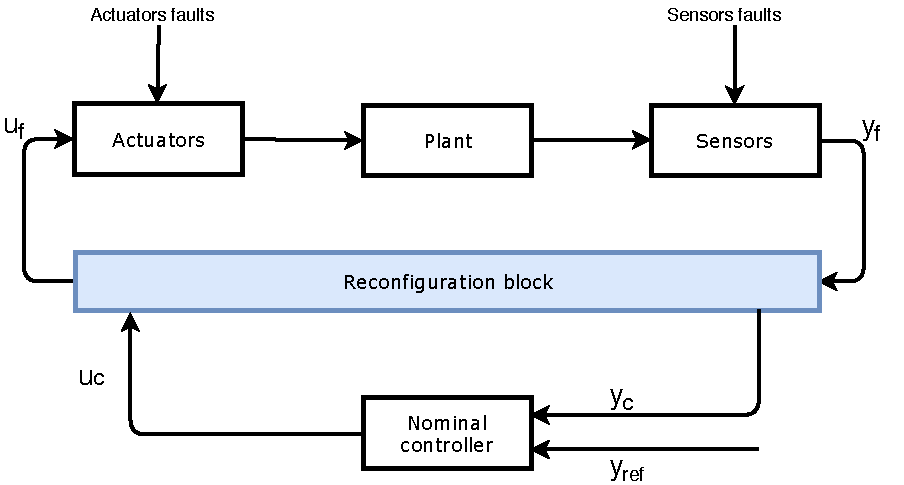
\includegraphics[width=0.8\linewidth]{figures/VirtualActuator}
 	\caption{ Virtual actuators and sensors scheme}
 	\label{fig:VA}
 \end{figure}
 
 The reconfiguration of the faulty actuators is made in the adequate actuator subsystems. 
 
 In the case of the reaction wheel subsystem compensation is needed, while in the magnetorquers not.
 
 In the case that a fault occurs in the reaction wheel sensor, the angular velocity measurement it is assumed functional and based on that measurement, the torque output from the faulty wheel can be computed. A second assumption is that the sensors will completely fail, but in this case a model of how the angular velocity of the wheel is decreasing over time is obtained. This model can be used as a virtual sensor for the angular velocity sensor. 
 
\section{Reaction Wheel Reconfiguration}
\label{sec:rwReconfig}
Fault handling in the redundant reaction wheel configuration can be done by isolating which is the reaction wheel where the fault occurred and shutting it off and redistributing the torques to the rest of the reaction wheels. Fault signals emitted by the fault detection modules are handled by the reconfiguration logic. Section \ref{ref:reactConfig} describes the distribution of reaction wheel torque demand between the reaction wheels. When the reconfiguration system receives a fault signal, it redistributes the $\vec{N_{rw}^d}$ torque demand by modifying $\underline{A}_M$ matrix in equation \ref{eq:transmatrix}. The torque demand for the faulty wheel becomes zero, while the sum of reaction wheel torques are controlled to follow $\vec{N_{rw}^d}$.

This reconfiguration/redistribution can be represented by changing the $\underline{A}_M$ columns corresponding to faulty wheels to zero vectors. For example, if a fault occurs in the 3rd reaction wheel, the transformation matrix becomes $\underline{A}_{M,f3}$, as presented in equation \ref{eq:ReactFault}.

\begin{equation}
	\label{eq:ReactFault}
	\underline{A}_{M,f3} = \begin{bmatrix}
		\vec{Axis^{M}_{1}}       & \vec{Axis^{M}_{2}}   & \vec{0}   & \vec{Axis^{M}_{4}} 
	\end{bmatrix} 
\end{equation}

\begin{figure}[H]
	\centering 
	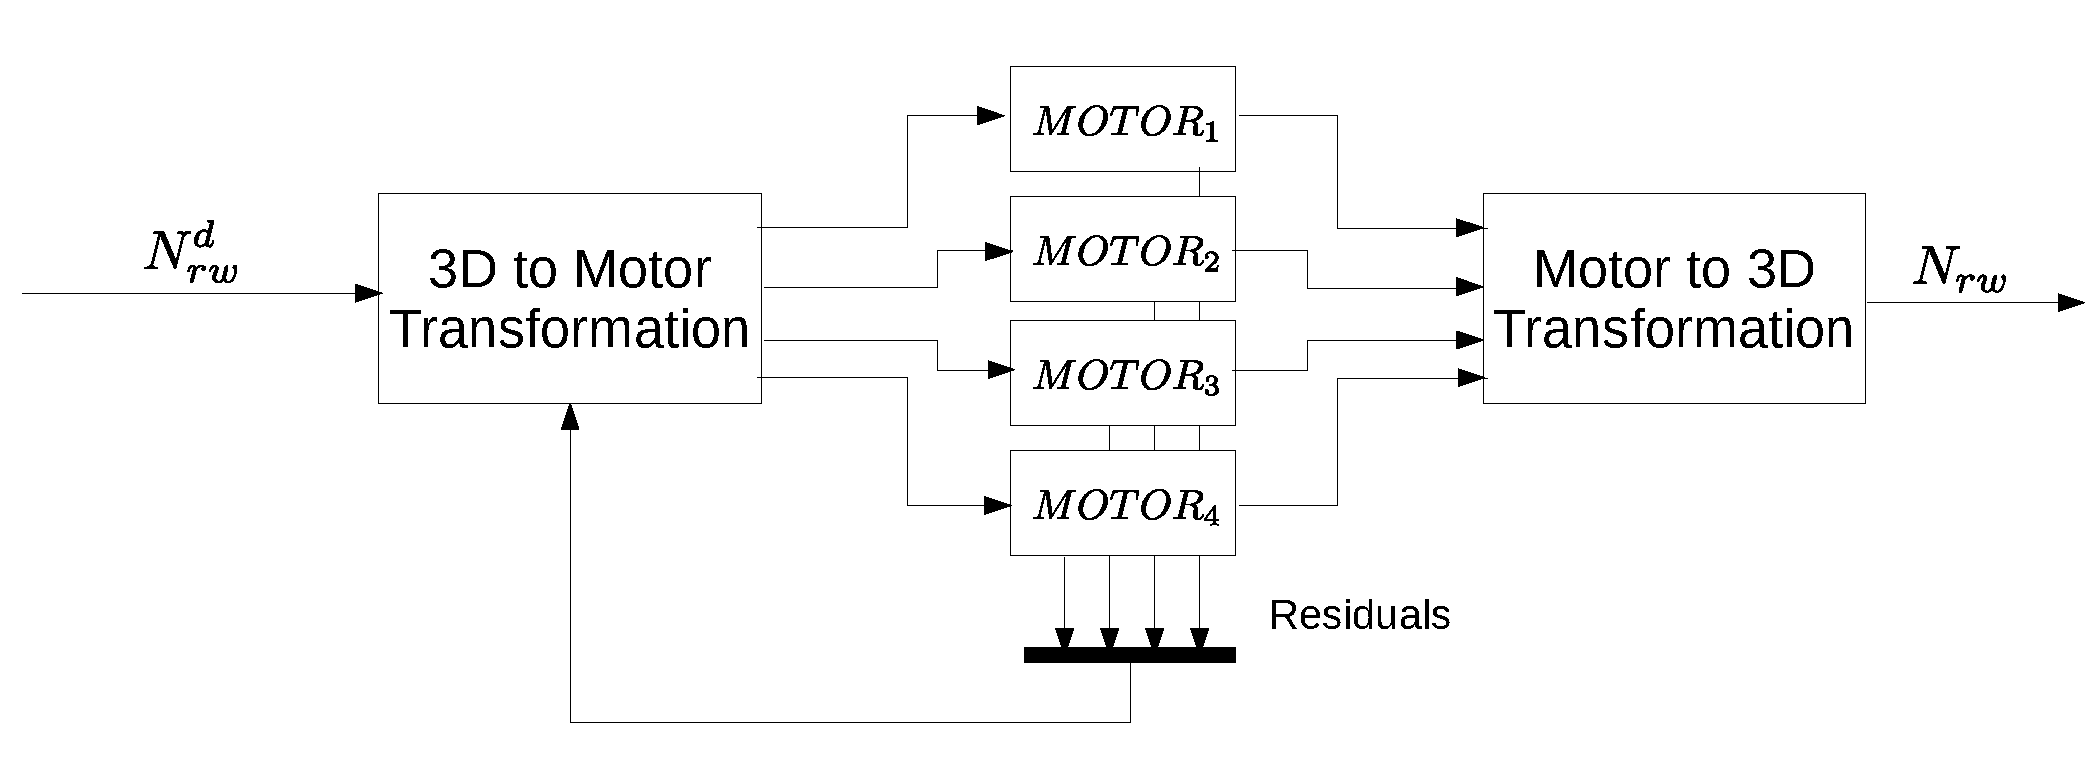
\includegraphics[width=170mm]{figures/reconfig.pdf}	
	\caption{Reconfiguration Control Scheme for Reaction Wheels}
	\label{fig:reconfig}
\end{figure}

\nomenclature[SA]{$\underline{A}_{M,fi}$}{Transformation matrix between axis oriented reaction wheel torque and torques in 3 dimensional body frame in case of faulty $i$th reaction wheel}

The pseudo inverse used for transformation between 3D to motor torque is calculated in the same manner as presented in equation \ref{eq:motorTrans}, see equation \ref{eq:motorTransFault}. The torque distribution controller scheme which checks for faults in the motors, is presented in Figure \ref{fig:reconfig}

\begin{equation}
	\label{eq:motorTransFault}
	\underline{A}_{M,f3}^\dagger   = \underline{A}_{M,f3}^T  (\underline{A}_{M,f3} \underline{A}_{M,f3}^T)^{-1}
\end{equation}
%
%\begin{figure}
%	\centering
%	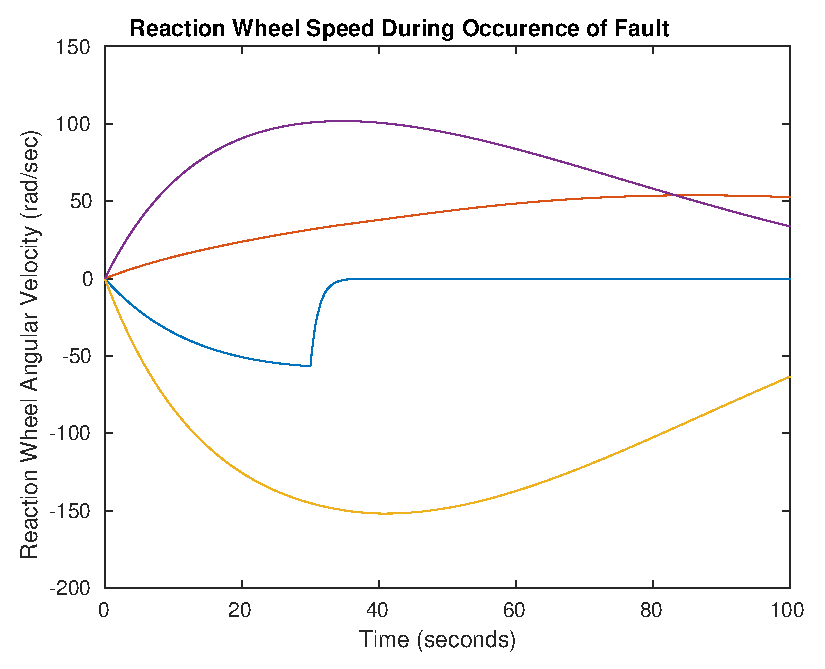
\includegraphics[width=120mm]{figures/residOmega}
%	\caption{Insert caption}
%	\label{fig:residualOmega}
%\end{figure} 

Equation \ref{eq:motorTransReconfig2} presents the reconfigured torque distribution equation.

\begin{equation}
\label{eq:motorTransReconfig2}
\vec{N_{M}^d} = \underline{A}_{M,f3}^\dagger \vec{N_{rw}^d}  
\end{equation}


\subsubsection{Reconfiguration with compensation in case of angular velocity sensor fault}



A reconfiguration scheme using anomaly detection in angular velocity sensors has been implemented in the simulation. The detection checks the magnitude of the angular velocity gradient, and if it's above the threshold, the supervisor shuts down the corresponding wheel in a controlled fashion and distributes the torque demand to the remaining wheels. This is necessary, since the reaction wheel control scheme relies on angular velocity measurements. 

It is imperative to compensate for the torque output of the faulty wheel for the satellite dynamics not to be affected by the fault. If the control voltage of the wheel is instantaneously turned off to zero at the moment the fault is detected, the torque output of the wheel can be quite large due to the fast deceleration, making compensation more problematic. Instead the control voltage should be decreased more slowly to reduce the torque output. The torque output of the faulty wheel can not be derived from angular velocity measurements in the presence of an angular velocity sensor fault. In order to be able to compensate for the deceleration torque, using the assumption that the only fault is in the sensor, wheel deceleration can be simulated based on the model, and compensation can be done for the simulated torque output of the wheel.

\begin{figure}
	\centering
	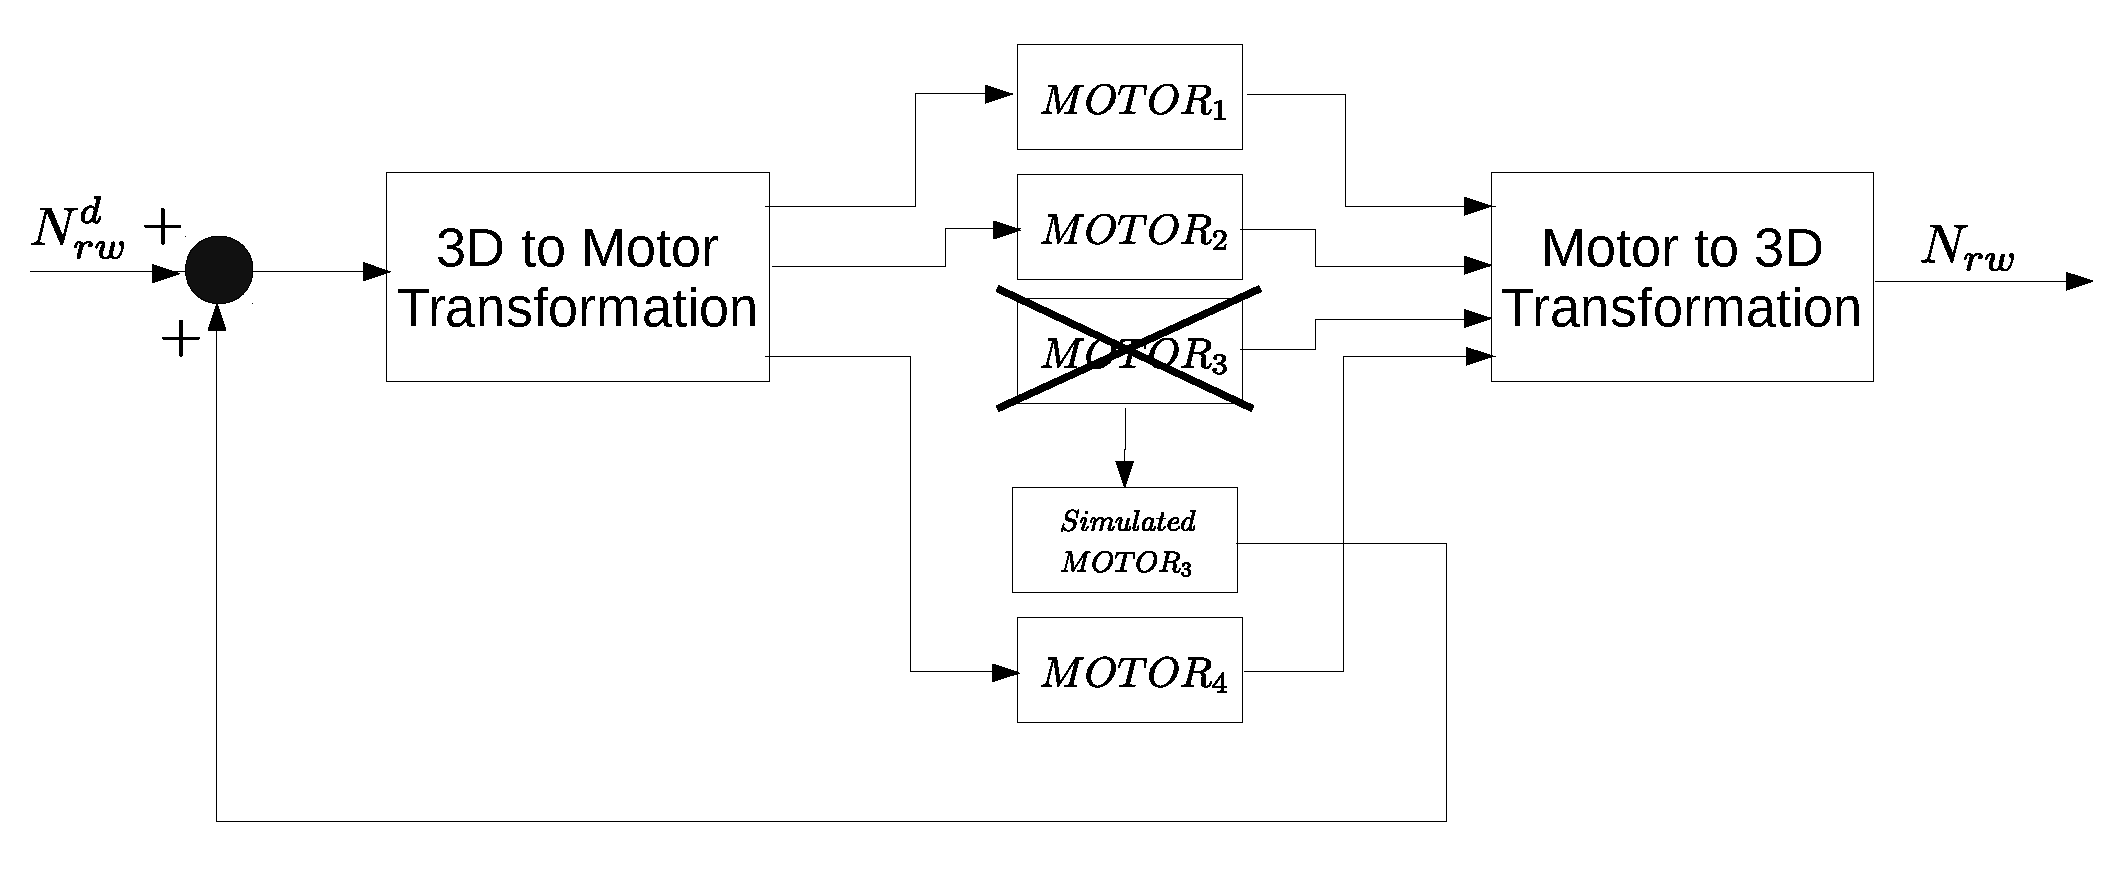
\includegraphics[width=120mm]{figures/simulatedCompensation}
	\caption{Shutdown torque compensation in case of angular velocity sensor fault.}
	\label{fig:angFaultCompensation}
\end{figure} 

The shut down happens as follows: when the sensor fault is detected, the system registers the momentary control voltage at the input of the faulty wheel, and starts slowly decreasing the voltage to zero. In parallel, a simulation starts for wheel deceleration with the angular velocity initial value being the last non-faulty value. The voltage input of the simulation is always the same as for the real system. As the fault occurs, the reaction wheel torque distribution is changed to omit the faulty wheel. The simulated torque output of the wheel faulty wheel is fed to the reaction wheel torque distributor for compensation, as shown in figure \ref{fig:angFaultCompensation}.

\begin{figure}
	\centering
	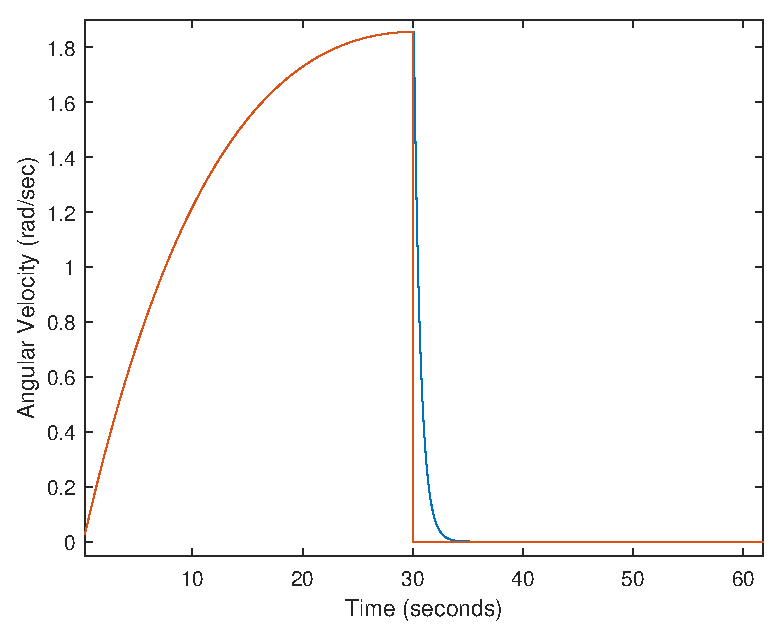
\includegraphics[width=120mm]{figures/omegaSensorfault_omega}
	\caption{$\omega_{M,i}$ sensor signal and actual value with fault occuring at 30 seconds}
\end{figure} 

\begin{figure}
	\centering
	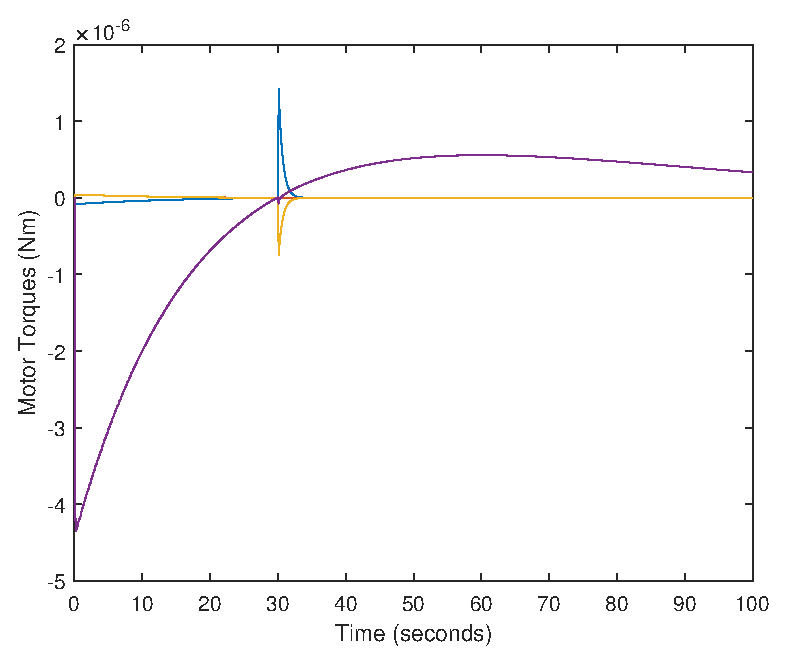
\includegraphics[width=120mm]{figures/omegaSensorfault_Nmotor}
	\caption{$N_M$ with $\omega$ sensor fault occuring at 20 seconds}
\end{figure} 

\begin{figure}
	\centering
	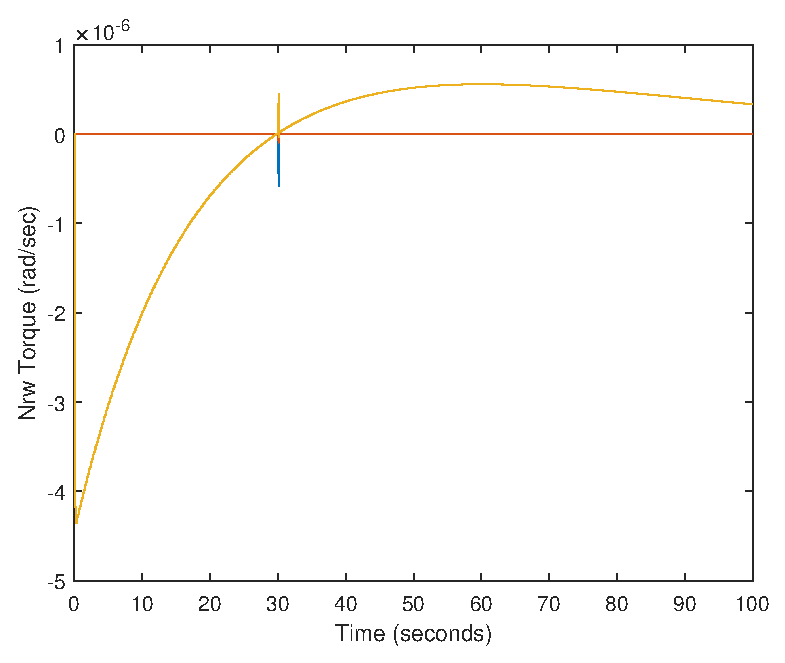
\includegraphics[width=120mm]{figures/omegaSensorfault_Nrw}
	\caption{$N_{rw}$ with $\omega$ sensor fault occuring at 20 seconds}
\end{figure} 



\subsubsection{Reconfiguration with compensation in case of residual fault detection}

If the structural analysis based motor fault detector discussed in section \ref{sec:structural} sends a fault signal, $\vec{\N_{rw}}$ is redistributed while the faulty wheel undergoes a controlled deceleration. The torque output of the faulty wheel is compensated for as shown in figure \ref{fig:resFaultCompensation}. One type of fault that the residual can detect is the change of the bearing friction. If the friction increases and the wheel is shutdown by cutting the control voltage to zero, the deceleration torque could become too large to compensate for. Instead, the reference angular velocity of the faulty wheel is smoothly decreased to zero, so that the faulty torque output stays small. Figures \ref{fig:resreconfig} - \ref{fig:resreconfig_ome} present the behaviour of the system during reconfiguration.

\begin{figure}
	\centering
	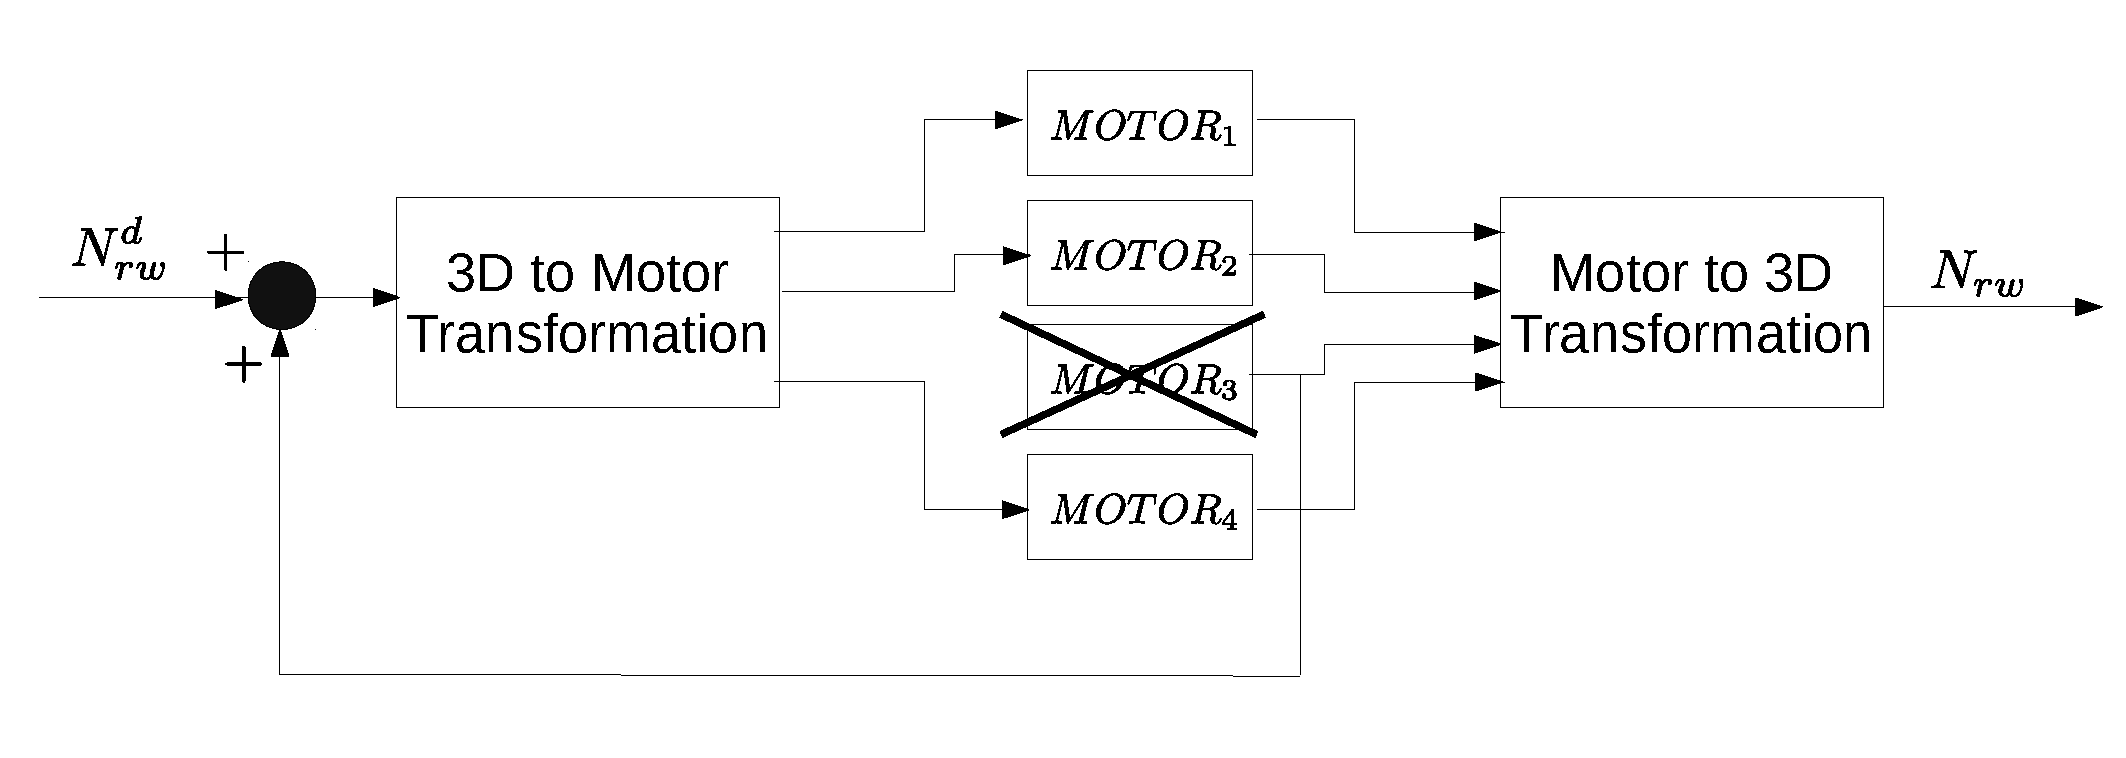
\includegraphics[width=120mm]{figures/residReconfigCompensation}
	\caption{Shutdown torque compensation in case of fault detected through residual.}
	\label{fig:resFaultCompensation}
\end{figure} 

%\begin{figure}
%	\centering
%	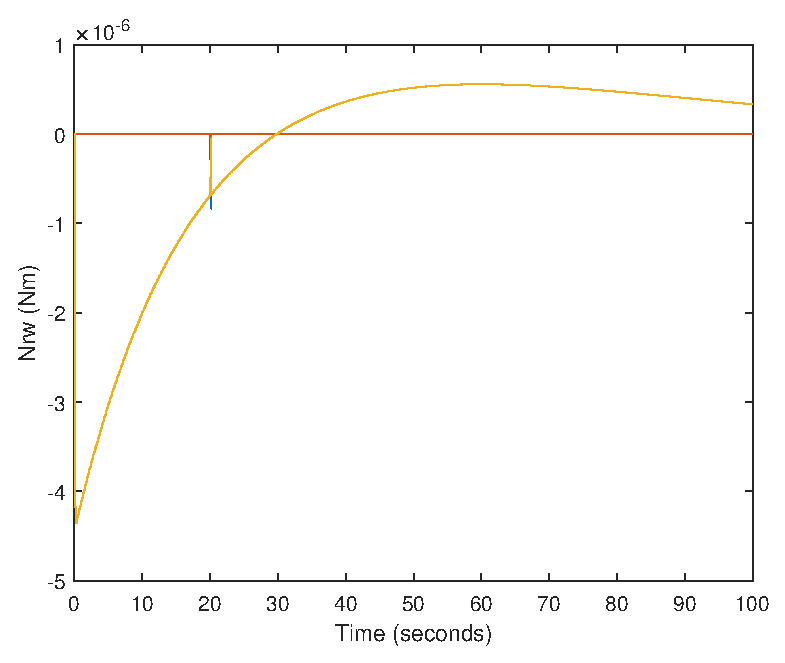
\includegraphics[width=120mm]{figures/3dTorque_resid_reconfig}
%	\caption{$N_rw$ with fault occuring at 20 seconds}
%\end{figure} 
%
%\begin{figure}
%	\centering
%	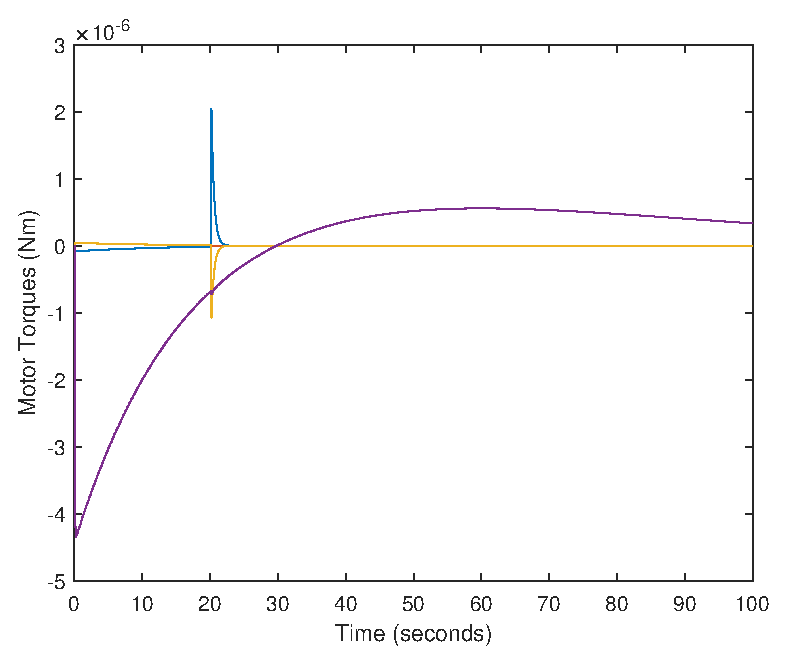
\includegraphics[width=120mm]{figures/torque_reconfig}
%	\caption{$N_M$ with fault occuring at 20 seconds}
%\end{figure} 
%
%\begin{figure}
%	\centering
%	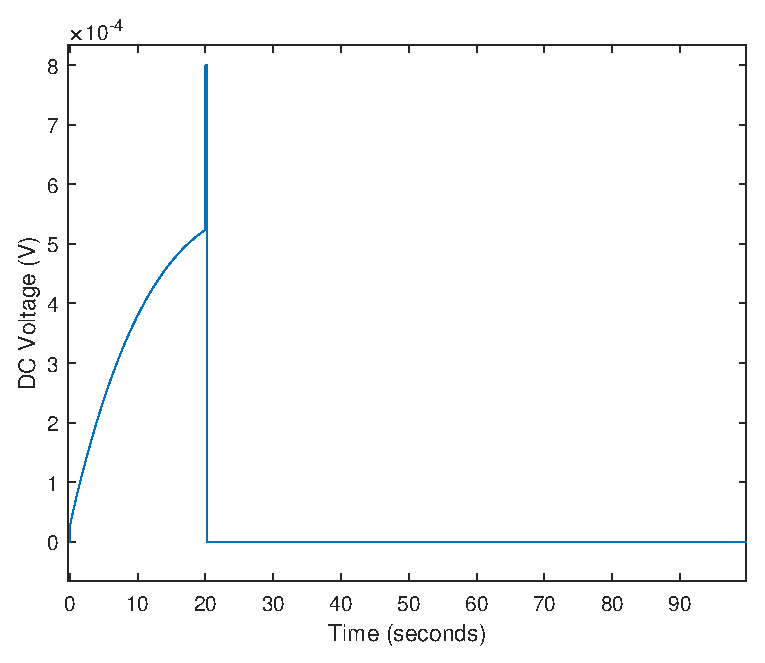
\includegraphics[width=120mm]{figures/voltage_reconfig}
%	\caption{Voltage control signal with fault occuring at 0 seconds}
%\end{figure} 
%
%
%\begin{figure}
%	\centering
%	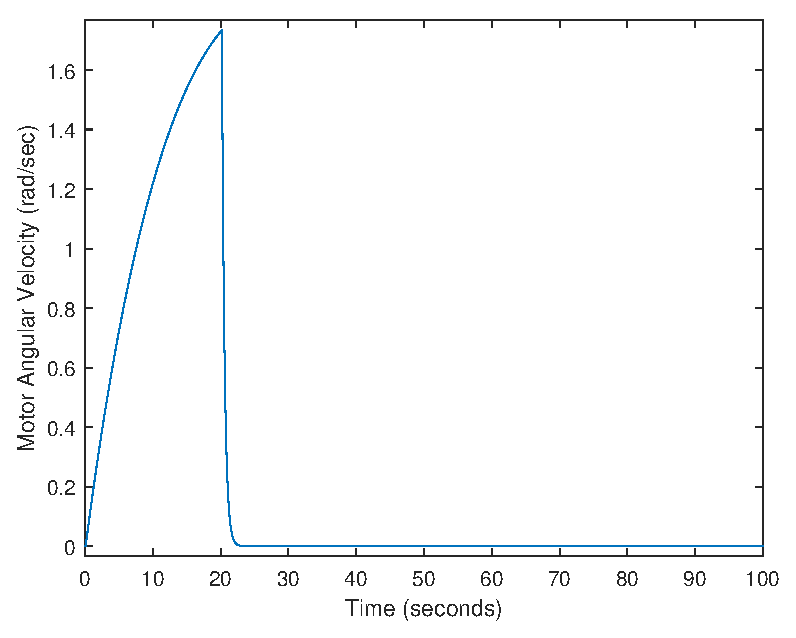
\includegraphics[width=120mm]{figures/omega_reconfig}
%	\caption{$\omega_{M,i}$ with fault occuring at 20 seconds}
%\end{figure} 
%
%
%\begin{figure}
%	\centering
%	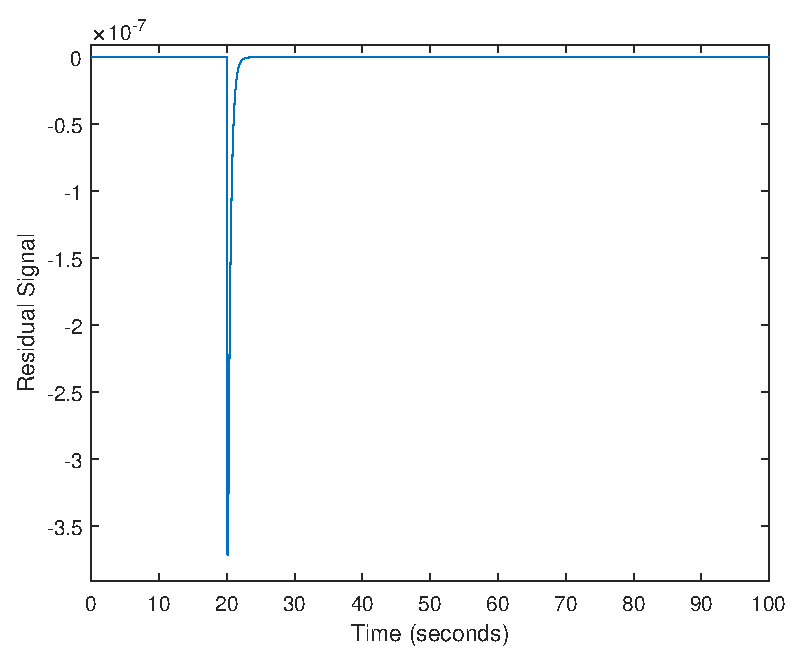
\includegraphics[width=120mm]{figures/residual_reconfig}
%	\caption{Residual signal with fault occuring at 20 seconds}
%\end{figure} 

\begin{figure}[H]
	\centering
	\begin{subfigure}{.5\textwidth}
	\centering
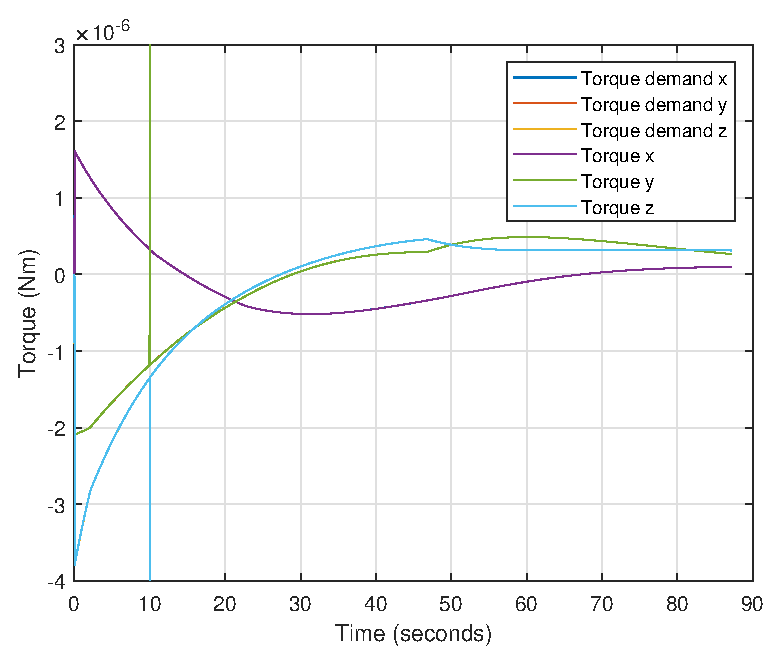
\includegraphics[width=70mm]{figures/smooth3dtorque}
\caption{}
	\label{fig:resreconfig_nrw}
	\end{subfigure}%
	\begin{subfigure}{.5\textwidth}
	\centering
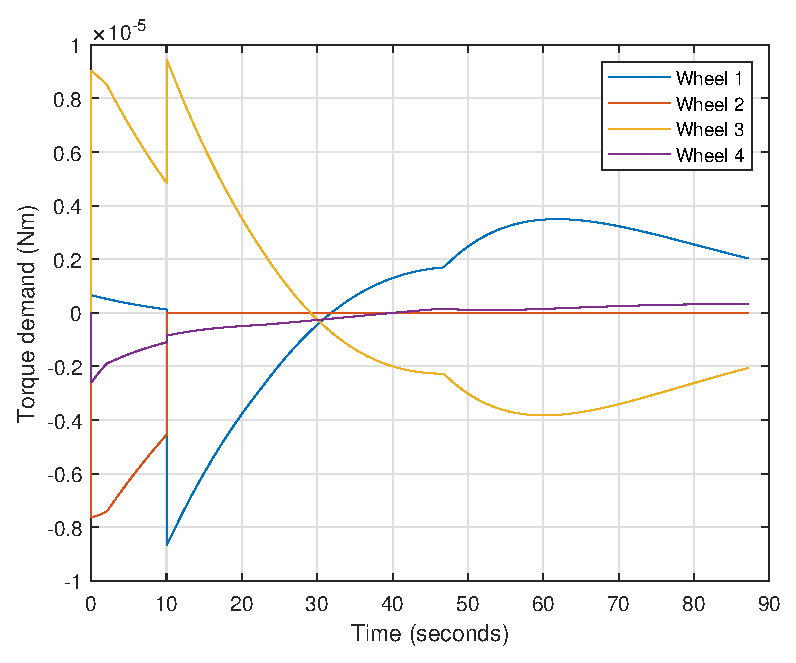
\includegraphics[width=70mm]{figures/smooth_motor_torque}
\caption{}
\label{fig:resreconfig_nm}
	\end{subfigure}
	\caption{Figure \ref{fig:resreconfig_nrw}: $N_{rw}$ with fault occuring at 10 seconds. Figure \ref{fig:resreconfig_nm}: $N_M$ with fault occuring at 10 seconds.}
	\label{fig:resreconfig}
\end{figure}

%\begin{figure}
%	\centering
%	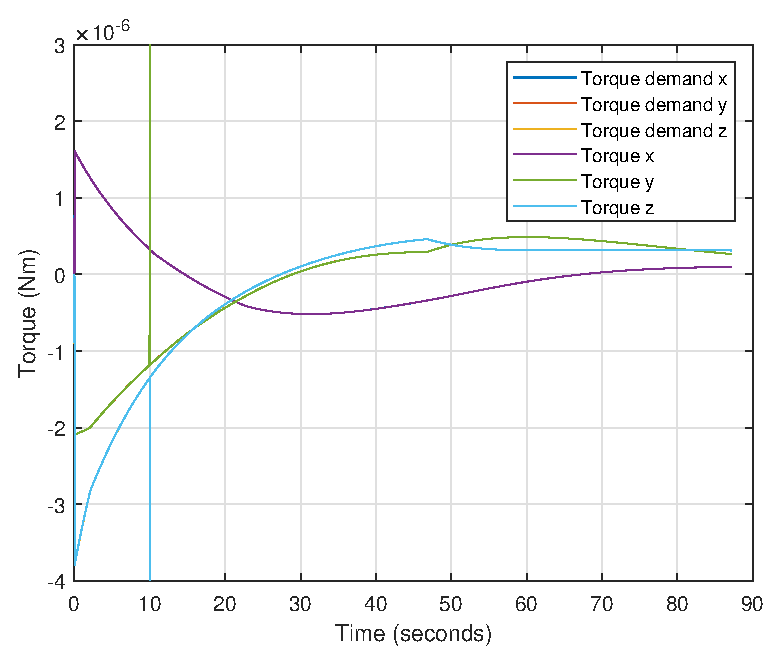
\includegraphics[width=120mm]{figures/smooth3dtorque}
%	\caption{$N_{rwn$ with fault occuring at 10 seconds}
%	\label{fig:resreconfig_nrw}
%\end{figure} 
%
%\begin{figure}
%	\centering
%	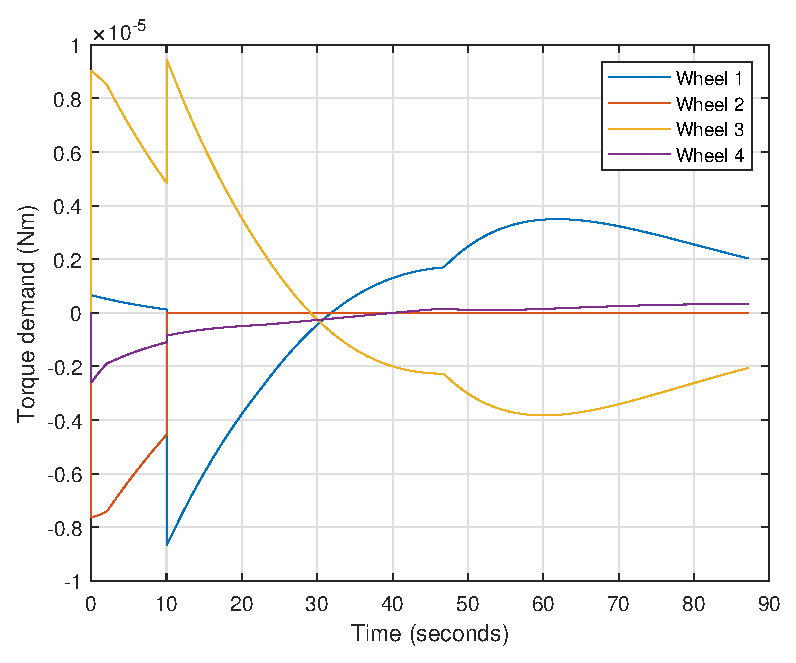
\includegraphics[width=120mm]{figures/smooth_motor_torque}
%	\caption{$N_M$ with fault occuring at 10 seconds}
%	\label{fig:resreconfig_nm}
%\end{figure} 

\begin{figure} [H]
\centering
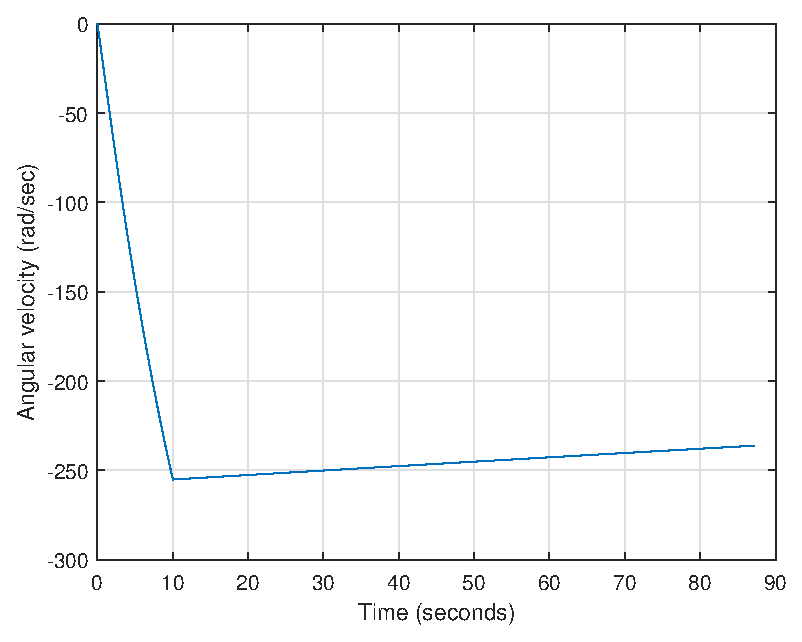
\includegraphics[width=70mm]{figures/smooth_omega_residual}
\caption{$\omega_{M,i}$ with fault occuring at 10 seconds}
\label{fig:resreconfig_ome}
\end{figure} 

\section{Magnetorquer Reconfiguration}
\label{sec:MTReconfig}

\subsubsection{Reconfiguration with compensation in case of Luenberger-like Observer residual fault detection}

Similarly to the reaction wheel reconfiguration \secref{sec:rwReconfig}, fault handling in the redundant magnetorquer scheme can be done by isolating the faulty magnetic component, shutting it off and at the same time turn on the redundant magnetorquer at the same axis. As it has been discussed in \secref{sec:simpleObserver} the Luenberger-like Observer is not robust in the sense of isolating which component is faulty. Therefore, a combination with the structural analysis method \secref{sec: MTStructAnal} can be  made in order to isolate the faulty component. Each method give a flag, commonly a binary input, such that when a fault is present each method indicate 1 and when a fault is absent indicate 0. Moreover, the structural analysis method is also limited on the faults which can detect. Therefore, the binary flags from both methods are inputs to a block which emulates the logic operator $OR$, so if the flags from each method give binary indicator 1, all the magnetorquers are switched which gives robustness in a manner of fault handling. In the \figref{fig:magneticconfig} it can be seen how the main magnetorquers shutting off in the presence of a fault in the power supply at time 150 and their corresponding pair takes action. Moreover, it is worth mentioning that isolation and configuration of only the faulty component can achieved by replacing the $OR$ by $AND$ logic operator, but this will lead in a reduced number of the family of faults that can be handled. 
%
%
%\begin{figure}[ht]  
%	\begin{minipage}{0.5\textwidth}
%		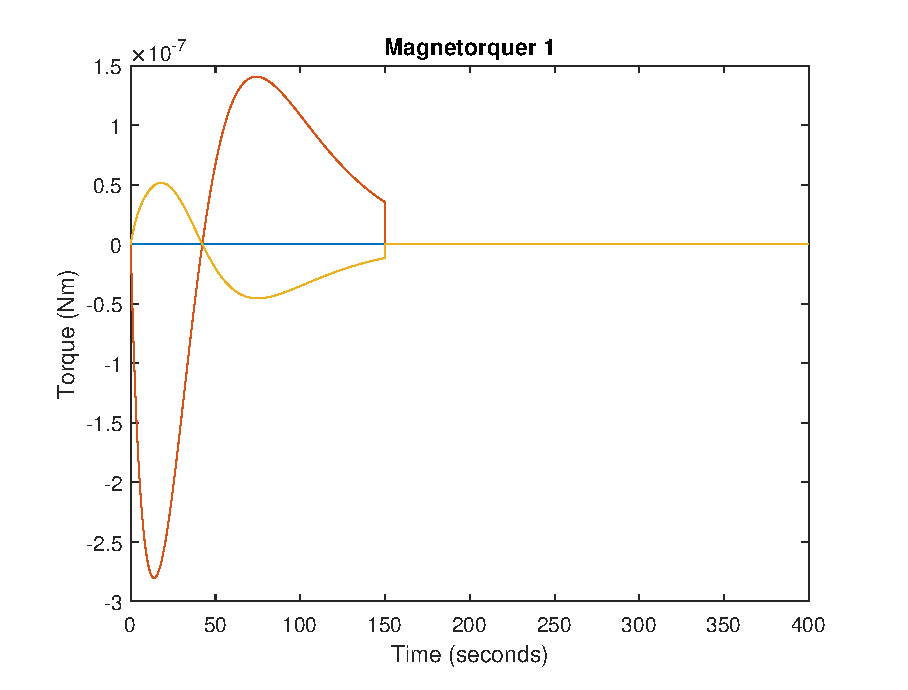
\includegraphics[width=\textwidth]{figures/config1.eps}
%	\end{minipage}
%	\hfill
%	\begin{minipage}{0.5\textwidth}
%		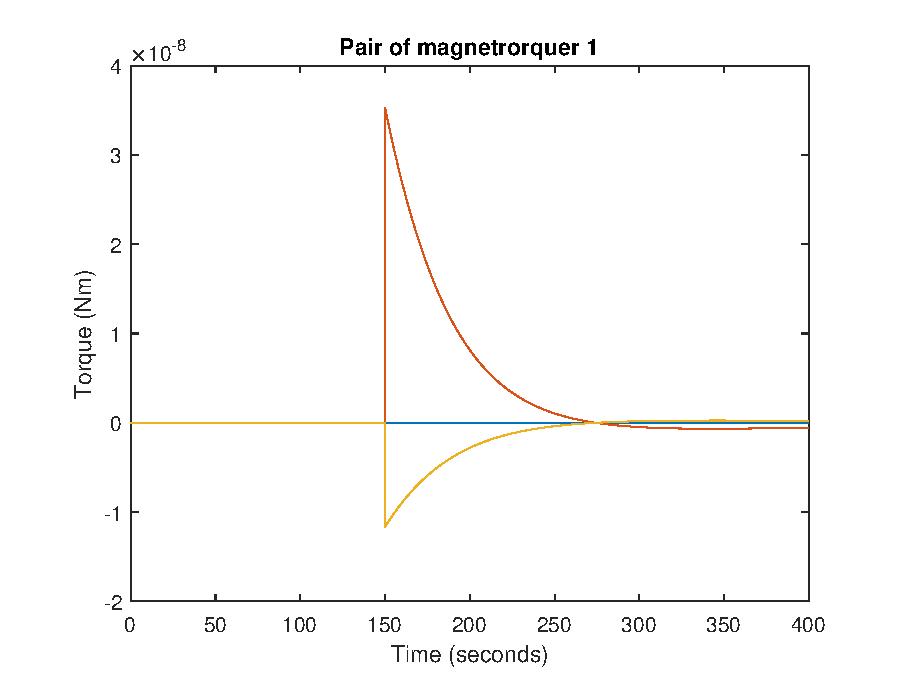
\includegraphics[width=\textwidth]{figures/config11.eps}
%	\end{minipage}
%\end{figure}
%\begin{figure}[ht]  
%	\begin{minipage}{0.5\textwidth}
%		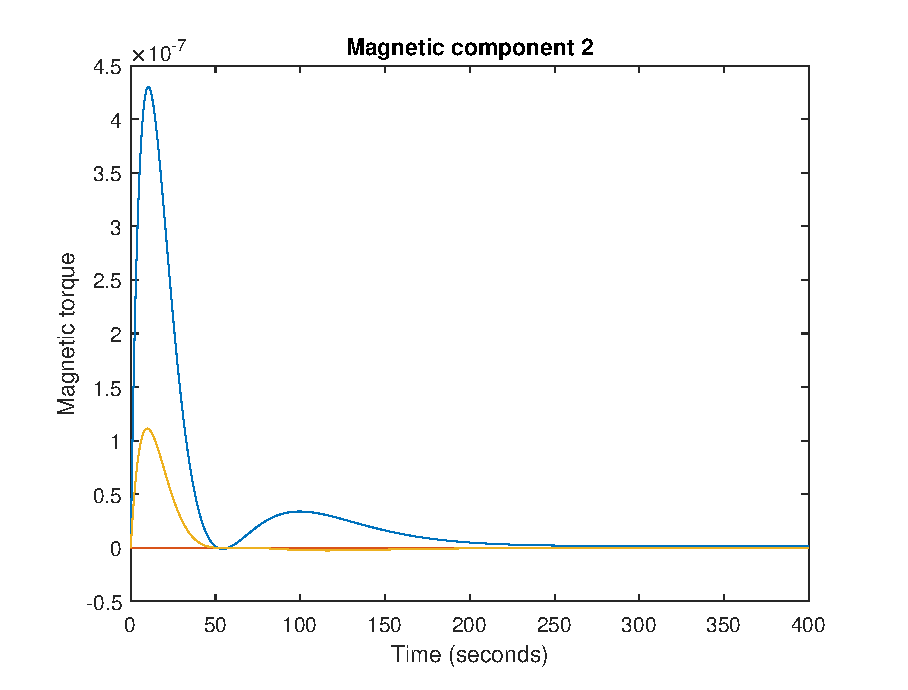
\includegraphics[width=\textwidth]{figures/config2.eps}
%	\end{minipage}
%	\hfill
%	\begin{minipage}{0.5\textwidth}
%		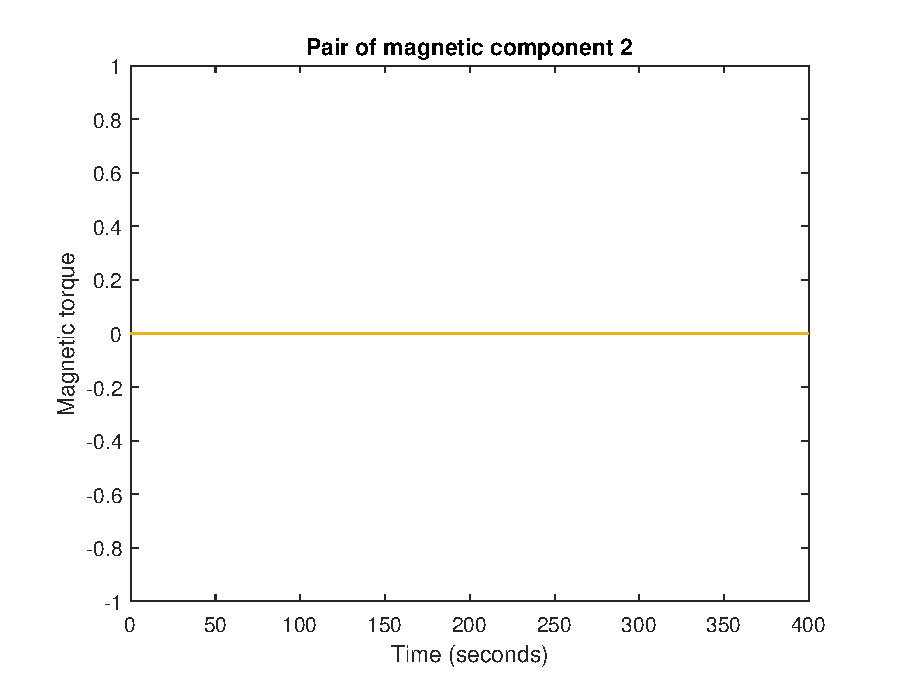
\includegraphics[width=\textwidth]{figures/config22.eps}
%	\end{minipage}
%\end{figure}    
%\begin{figure}[ht]  
%	\begin{minipage}{0.5\textwidth}
%		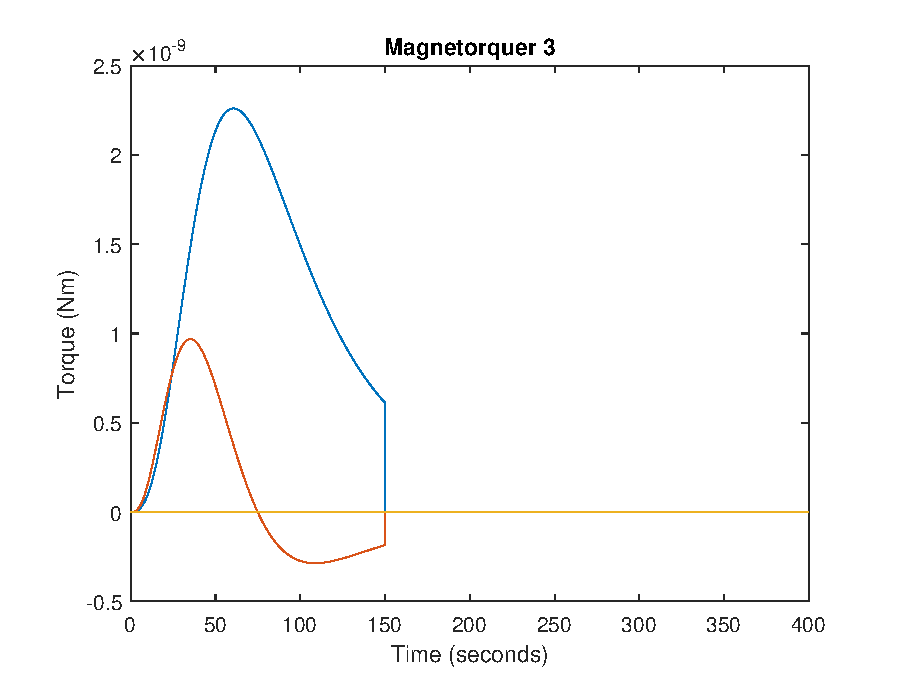
\includegraphics[width=\textwidth]{figures/config3.eps}
%	\end{minipage}
%	\hfill
%	\begin{minipage}{0.5\textwidth}
%		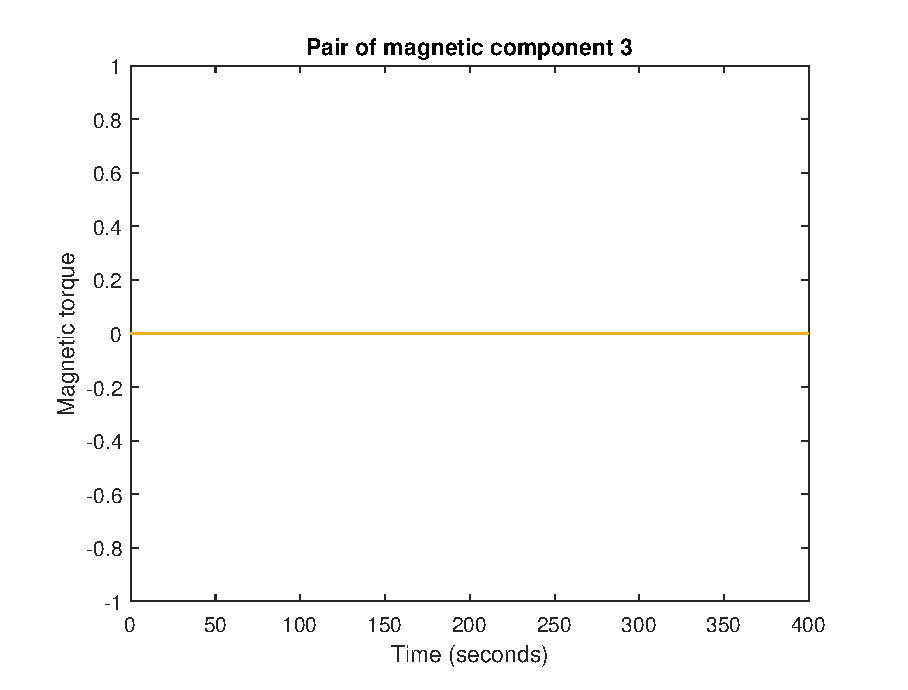
\includegraphics[width=\textwidth]{figures/config33.eps}
%	\end{minipage}
%	\caption{To the left are depicted the magnetorquers of each axis subjected to a fault in the voltage supply and to the right the redundant magnetorquer pairs}
%	\label{fig:magneticconfig}
%\end{figure}  
%%

\begin{figure}[H]
	\begin{subfigure}{0.5\linewidth}
		\centering
		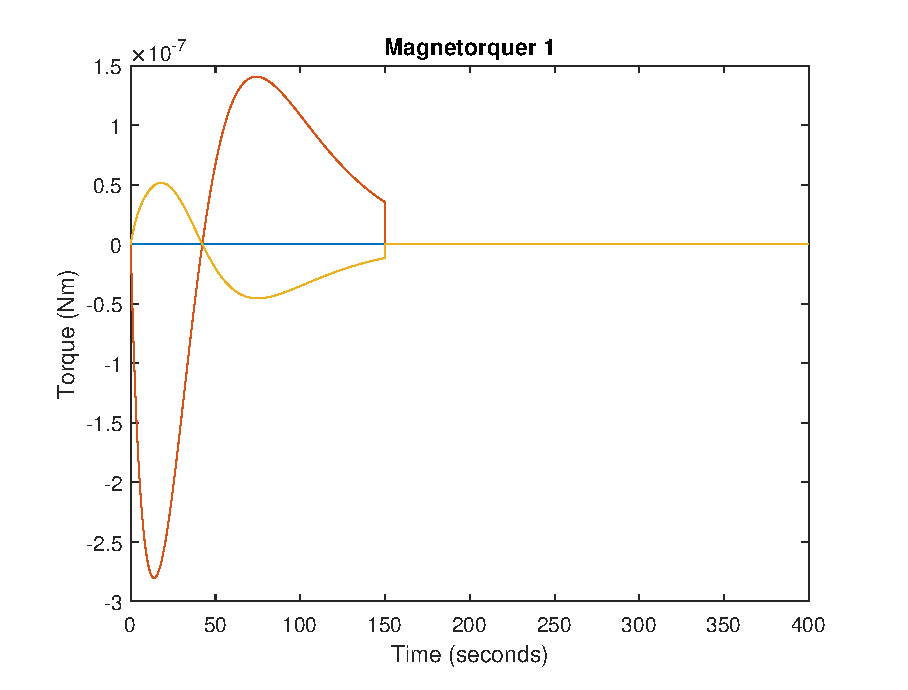
\includegraphics[width=1\linewidth]{figures/config1.eps}
		\label{fig:magcompens}
	\end{subfigure}
	\begin{subfigure}{0.5\linewidth}
		\centering
		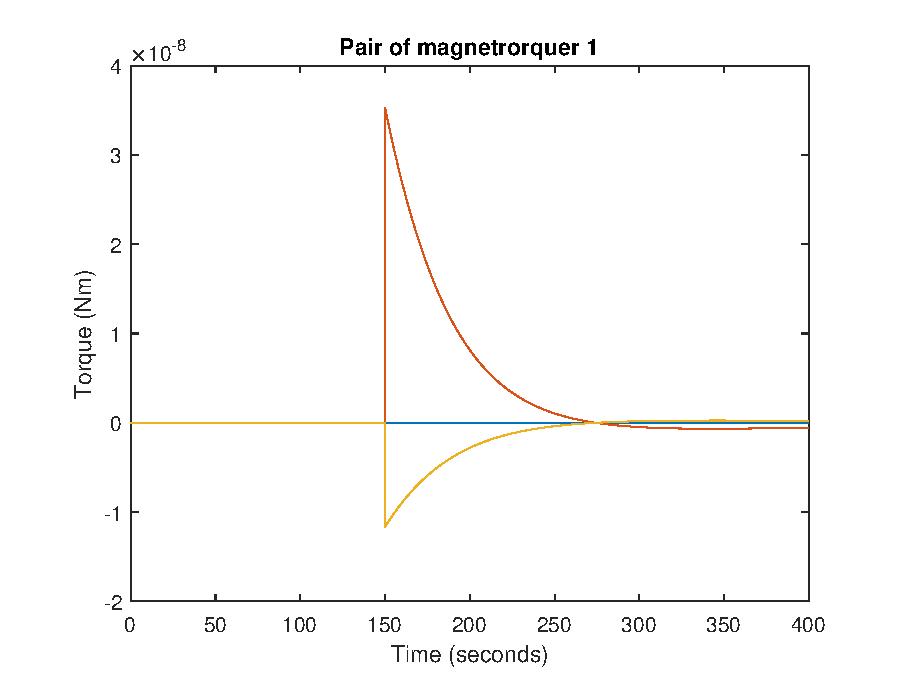
\includegraphics[width=1\linewidth]{figures/config11.eps}
		\label{fig:fig:magcompens2}	
	\end{subfigure}
\begin{subfigure}{0.5\linewidth}
	\centering
	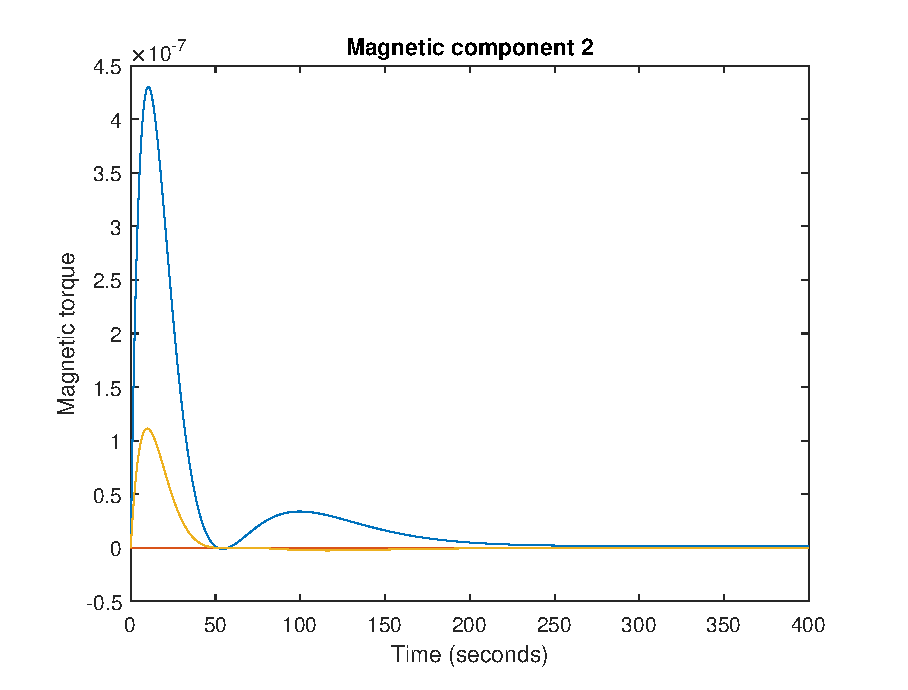
\includegraphics[width=1\linewidth]{figures/config2.eps}
	\label{fig:fig:magcompens3}
\end{subfigure}
\begin{subfigure}{0.5\linewidth}
	\centering
	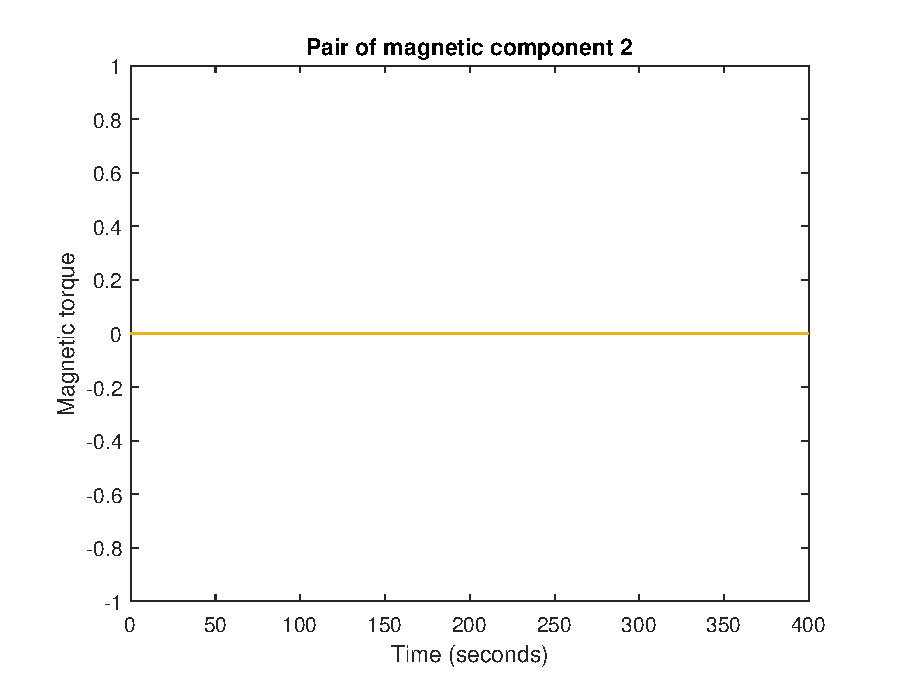
\includegraphics[width=1\linewidth]{figures/config22.eps}
	\label{fig:fig:magcompens4}	
\end{subfigure}
\begin{subfigure}{0.5\linewidth}
	\centering
	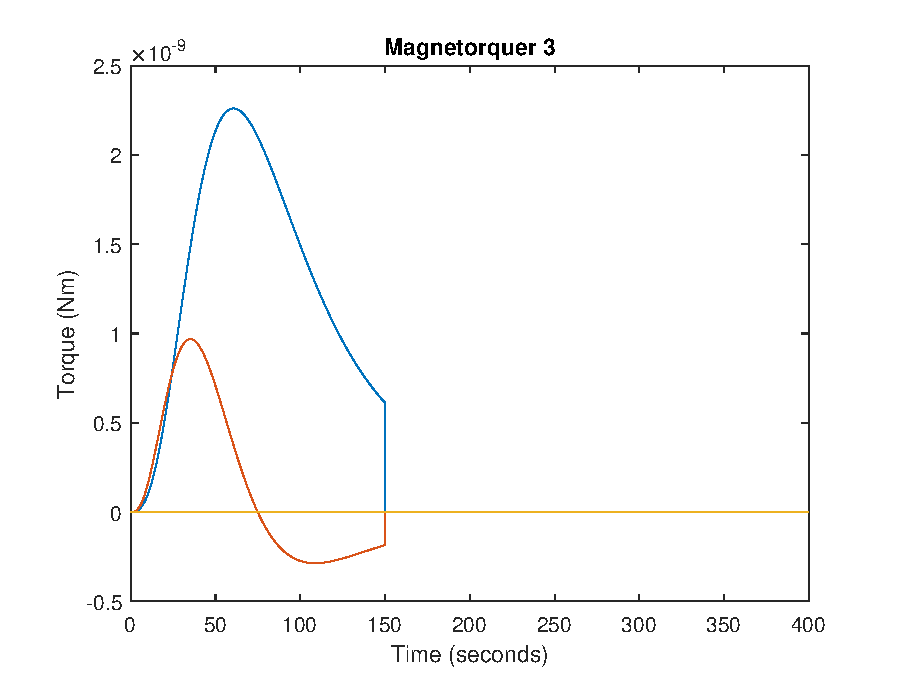
\includegraphics[width=1\linewidth]{figures/config3.eps}
	\label{fig:fig:magcompens33}
\end{subfigure}
\begin{subfigure}{0.5\linewidth}
	\centering
	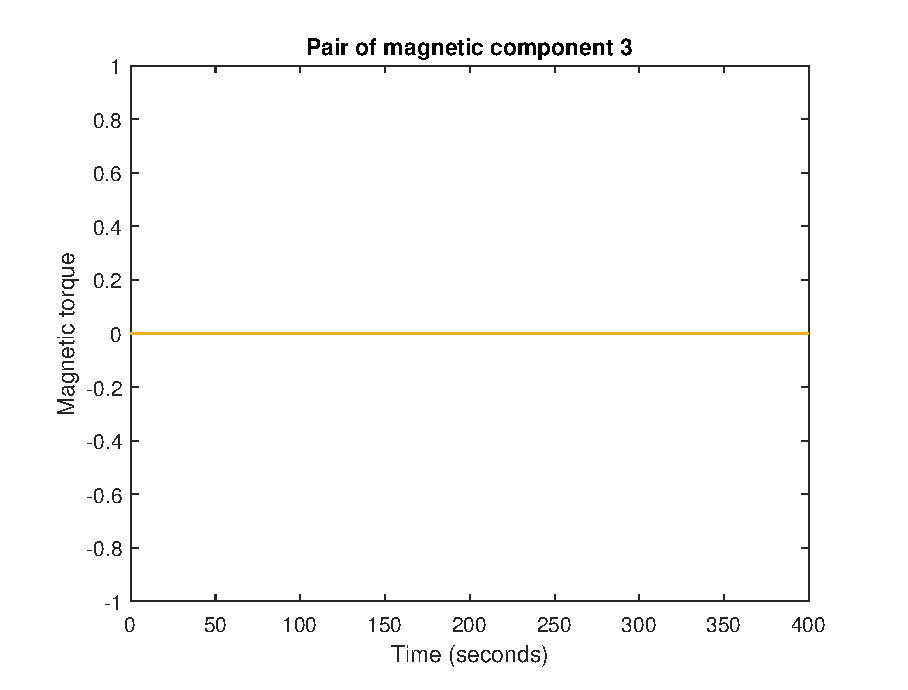
\includegraphics[width=1\linewidth]{figures/config33.eps}
	\label{fig:fig:magcompens43}	
\end{subfigure}
	\caption{To the left are depicted the magnetorquers of each axis subjected to a fault in the voltage supply and to the right the redundant magnetorquer pairs.}
	\label{fig:magneticconfig}
\end{figure}

